%%
%% getstart.tex -- Flight Gear documentation: The FlightGear Manual
%% Chapter file
%%
%% Written by Michael Basler, started September 1998.
%%
%% Copyright (C) 2002 Michael Basler
%%
%%
%% This program is free software; you can redistribute it and/or
%% modify it under the terms of the GNU General Public License as
%% published by the Free Software Foundation; either version 2 of the
%% License, or (at your option) any later version.
%%
%% This program is distributed in the hope that it will be useful, but
%% WITHOUT ANY WARRANTY; without even the implied warranty of
%% MERCHANTABILITY or FITNESS FOR A PARTICULAR PURPOSE.  See the GNU
%% General Public License for more details.
%%
%% You should have received a copy of the GNU General Public License
%% along with this program; if not, write to the Free Software
%% Foundation, Inc., 675 Mass Ave, Cambridge, MA 02139, USA.
%%
%% $Id: preface.tex,v 0.6 2002/09/09 michael
%% (Log is kept at end of this file)

%%%%%%%%%%%%%%%%%%%%%%%%%%%%%%%%%%%%%%%%%%%%%%%%%%%%%%%%%%%%%%%%%%%%%%%%%%%%%%%%%%%%%%%%%%%%%%%
\chapter*{Preface\label{preface}}
%%%%%%%%%%%%%%%%%%%%%%%%%%%%%%%%%%%%%%%%%%%%%%%%%%%%%%%%%%%%%%%%%%%%%%%%%%%%%%%%%%%%%%%%%%%%%%%

\begin{figure}[!htp]
\centering
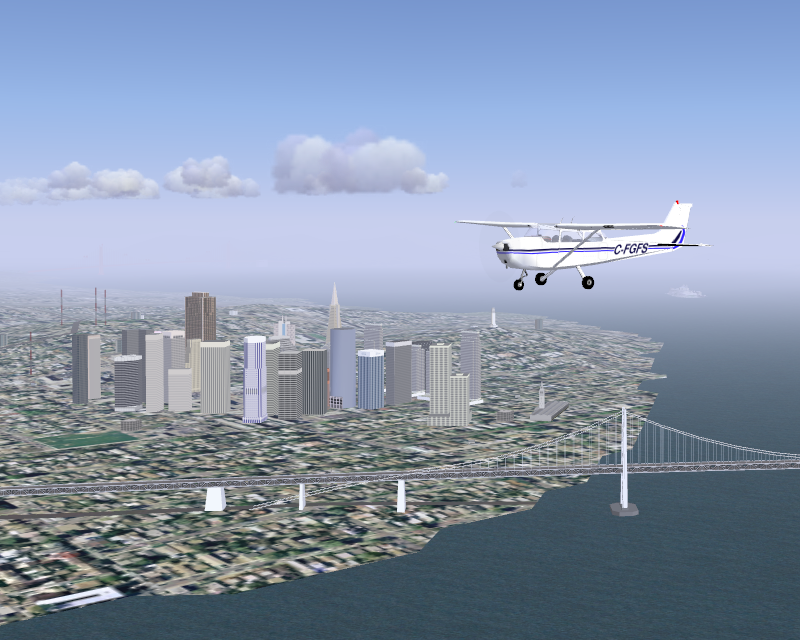
\includegraphics[width=0.75\textwidth]{img/preface.png}
\caption{Cessna 172 near San Francisco}
\end{figure}


\FlightGear{} is a free Flight Simulator developed cooperatively over the Internet 
by a group of flight simulation and programming enthusiasts. "The
FlightGear Manual" is meant to give beginners a guide in getting
\FlightGear{} up and running, and themselves into the air. It is not
intended to provide complete documentation of all the features and
add-ons of \FlightGear{} but, instead, aims to give a new user the best
start to exploring what \FlightGear{} has to offer.

This version of the document was written for \FlightGear{} version 0.9.11. 
Users of earlier versions of \FlightGear{} will still find this document
useful, but some of the features described may not be present.

This guide is split into three parts and is structured as follows.

\medskip

\noindent
\textbf{Part I: Installation}
\medskip

 \noindent
Chapter~\ref{free}, \textit{Want to have a free flight? Take \FlightGear{}}, introduces
\FlightGear{}, provides background on the philosophy behind it and describes the system requirements.
 \medskip

 \noindent
In Chapter~\ref{prefligh}, \textit{Preflight: Installing \FlightGear{}}, you will find
instructions for installing the binaries\index{binary distribution} and additional scenery and aircraft. 
 \medskip

\noindent
\textbf{Part II: Flying with \FlightGear{}}
\medskip

 \noindent
  The following Chapter~\ref{takeoff}, \textit{Takeoff: How to start
  the program}, describes how to actually start the installed program.
  It includes an overview on the numerous command line options as well
  as configuration files.
 \medskip

 \noindent
  Chapter~\ref{flight}, \textit{In-flight: All about instruments,
  keystrokes and menus}, describes how to operate the program, i.\,e\.
  how to actually fly with \FlightGear{}\hspace{-1mm}. This includes a
  (hopefully) complete list of pre-defined keyboard commands, an
  overview on the menu entries, detailed descriptions on the instrument
  panel and HUD (head up display), as well as hints on using the mouse
  functions.
 \medskip

 \noindent
  Chapter~\ref{features}, \textit{Features} describes some of the special
  features that \FlightGear{} offers to the advanced user.
 \medskip

\noindent
\textbf{Part III: Tutorials}
\medskip

 \noindent
 Chapter~\ref{tutorials}, \textit{Tutorials},
provides information on the many tutorials available for new pilots.
 \medskip

 \noindent
 Chapter~\ref{basic}, \textit{A Basic Flight Simulator Tutorial},
provides a tutorial on the basics of flying, illustrated with many
examples on how things actually look in \FlightGear{}.
 \medskip

 \noindent
 Chapter~\ref{crosscountry}, \textit{A Cross Country Flight Tutorial},
describes a simple cross-country flight in the San Fransisco area that
can be run with the default installation.
 \medskip

 \noindent
 Chapter~\ref{ifr}, \textit{An IFR Cross Country Flight Tutorial},
describes a similar cross-country flight making use of the instruments to 
successfully fly in the clouds under Instrument Flight Rules (IFR).
 \medskip

\noindent
\textbf{Appendices}
\medskip

 \noindent
  In Appendix~\ref{missed}, \textit{Missed approach: If anything refuses to work},
   we try to help you work through some common problems faced when using \FlightGear{}.
 \bigskip

 \noindent
Appendix~\ref{opengl}, \textit{OpenGL graphics drivers}, describes some
special problems you may encounter in case your system lacks support
for the OpenGL graphics API \Index{OpenGL} which \FlightGear{} is based
on.
 \medskip

 \noindent
 Appendix~\ref{building}, \textit{Building the plane: Compiling the program},
explains how to build (compile and link) the simulator. Depending on your platform this
may or may not be required. 
 \medskip

 \noindent
  In the final Appendix~\ref{landing}, \textit{Landing: Some further thoughts before leaving the plane}, we would like to give credit to those who deserve it, sketch an overview
on the development of \FlightGear and point out what remains to be done.
 \medskip

 \noindent
 Accordingly, we suggest reading the Chapters as follows:
 \medskip


\noindent
\begin{tabular}{ll}
 \textbf{Installation}                                  	&\\
 Users of binary distributions (notably under Windows):	 	&~\ref{prefligh}\\
 Installation under Linux/UNIX:               			&~\ref{building},~\ref{prefligh}\\
 Installation under Macintosh:               			&~\ref{prefligh}\\
  \textbf{Operation}                           			& \\
 Program start (all users):                      		&~\ref{takeoff}\\
 Keycodes, Panel, Mouse\ldots (all users):       		&~\ref{flight}\\
 \textbf{Troubleshooting}                      				& \\
 General issues:																						&~\ref{missed}\\
 Graphics problems: 									            				&~\ref{opengl}\\
 \textbf{Optionally}                           						&~\ref{free},~\ref{landing} 
\end{tabular}
\bigskip

\noindent
 While this introductory guide is meant to be self contained, we strongly suggest having a look into further documentation, especially in case of trouble:

\begin{itemize}
 \item For additional hints on troubleshooting and more, \textbf{please read the FAQ}\index{FAQ} 
 \medskip

 \noindent
 \web{http://www.flightgear.org/Docs/FlightGear-FAQ.html},
 
 The FAQ contains a host of valuable information, especially on rapidly changing flaws and additional reading, thus we strongly suggest consulting it in conjunction with our guide.
 
 
 \item A handy \textbf{leaflet}\index{leaflet} on operation for printout is available at
 \medskip

 \noindent
 \web{http://www.flightgear.org/Docs/InstallGuide/FGShortRef.html},
 \item Additional user documentation on special aspects is available within the base package under the directory \texttt{/FlightGear/Docs}.
 
 \item There is an official \FlightGear{} \textbf{wiki}\index{wiki} available at
 \medskip
 \noindent
 \web{http://wiki.flightgear.org},
 \end{itemize}

\noindent 
Finally:
\medskip


We know most people hate reading manuals. If you are sure the graphics driver for your card supports \Index{OpenGL} (check documentation; for instance all \Index{NVIDIA} Windows and Linux drivers for \Index{TNT}/TNT2/\Index{Geforce}/Geforce2/Geforce3 do) and if you are using one of the following operating systems:

\begin{itemize}
\item \Index{Windows} 95/98/ME/NT/2000/XP,
\item \Index{Macintosh} Mac OSX
\item \Index{Linux}
\item \Index{SGI Irix}
\end{itemize}

 \noindent
you can possibly skip at least Part I of this manual and exploit the pre-compiled binaries\index{binaries!pre-compiled}. These as well as instructions on how to set them up, can be found at
 \medskip

\web{http://www.flightgear.org/Downloads/}.
 \medskip

 \noindent
In case you are running \FlightGear{} on Linux, you may also be able to get binaries bundled with your distribution. Several vendors already include \FlightGear{} binaries into their distributions.
 
Just download them, install them according to the description and run them via the installed FlightGear icon (on Windows), or texttt{fgfs} having set the environmental variables described in Chapter \ref{takeoff} (on Linux).

There is no guarantee for this approach to work, though. If it doesn't, don't give up! Have a closer look through this guide notably Section~\ref{prefligh} and be sure to check out the \Index{FAQ}.


%% Revision 0.00  1998/09/08  michael
%% Initial revision for version 0.41.
%% Revision 0.01  2002/01/01 michael
%% Included outline of the Guide, integrated former separate chapter ''Quickstart''
%% revision 0.5 2002/01/01 michael/martin
%% Hint on Linux distros
%% revision 0.6 2002/09/09 michael
%% minor corrections
%% revision 0.7 2005/11.10 stuart
%% Changes for moving compilation information to appendix
